\begin{pastexam}[label={px:gk3-100-ds-08}]{高考三級資訊處理 100 年 第八題}
（申論；10 分）

輸入 10000 個字元，其中字元出現次數：\#(A)=1400，\#(B)=800，\#(C)=3000，\#(D)=2700，\#(E)=600，\#(F)=1500，
\#(其他字母)=0。使用霍夫曼（Huffman）編碼進行壓縮，其壓縮結果不含編碼簿（codebook）需要多少 bits？（10 分）
\end{pastexam}

\begin{pastsoln}
答案：$24200$ bits。

\textbf{建樹}（資結書第~19.3~節、虛擬碼~19.3）：每次取出次數最小的兩個合併，新節點的次數是兩者之和。
\begin{enumerate}
\item E(600)、B(800) 合併成 $1400$。
\item A(1400)、$\{E,B\}$(1400) 合併成 $2800$。
\item F(1500)、D(2700) 合併成 $4200$。
\item $\{A,E,B\}$(2800)、C(3000) 合併成 $5800$。
\item $4200$、$5800$ 合併成 $10000$，是根。
\end{enumerate}
\begin{center}
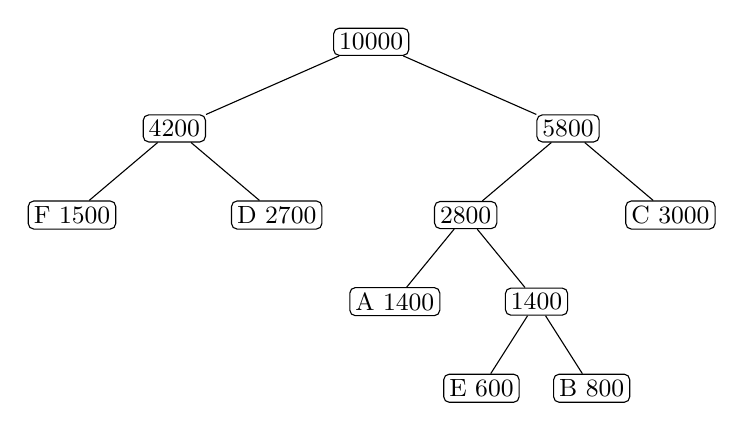
\begin{tikzpicture}[every node/.style={draw,rounded corners=2pt,inner sep=2pt,font=\small},
  level distance=11mm, level 1/.style={sibling distance=50mm}, level 2/.style={sibling distance=26mm},
  level 3/.style={sibling distance=18mm}, level 4/.style={sibling distance=14mm},
  edge from parent/.style={draw}]
\node {10000}
  child {node {4200} child {node {F 1500}} child {node {D 2700}}}
  child {node {5800}
    child {node {2800} child {node {A 1400}} child {node {1400} child {node {E 600}} child {node {B 800}}}}
    child {node {C 3000}}};
\end{tikzpicture}
\end{center}

\textbf{碼長與總長。} 碼長等於葉子的深度：F、D、C 是 $2$，A 是 $3$，E、B 是 $4$。
\[
\begin{aligned}
&1500 \cdot 2 + 2700 \cdot 2 + 3000 \cdot 2 + 1400 \cdot 3 + 600 \cdot 4 + 800 \cdot 4 \\
&= 3000 + 5400 + 6000 + 4200 + 2400 + 3200 = 24200 \text{ bits}.
\end{aligned}
\]
也可以把每次合併的和加起來（資結書引理~19.6）：$1400 + 2800 + 4200 + 5800 + 10000 = 24200$。 第 2 步
A 和 $\{E,B\}$ 都是 $1400$，誰當左右、跟誰合併的平手選法不同，碼可能不同，但總長一定是 $24200$。
對照：$6$ 種字元用固定長度要 $\lceil \lg 6 \rceil = 3$ bits，共 $30000$ bits。
\end{pastsoln}
